%-------------------------------------------------------------
% Filename : ECE569_Project_Final_Report_Group7.tex
% Authors  : Mason Edgar, Angel Silva, Peter Rulkov
% Course   : ECE 569
% Semester : Spring 2024
%-------------------------------------------------------------
\documentclass[conference]{IEEEtran}
\usepackage{cite}
\usepackage{bm}
\usepackage{mathtools}
\usepackage{amssymb, amsfonts}
\usepackage{algorithmic}
\usepackage{graphicx}
\usepackage{textcomp}
\usepackage{xcolor}
\usepackage{nameref}
\usepackage{subfig}
\usepackage{listings}
\usepackage[hidelinks]{hyperref}
%---
\def\BibTeX{{\rm B\kern-.05em{\sc i\kern-.025em b}\kern-.08em T\kern-.1667em\lower.7ex\hbox{E}\kern-.125emX}}
\graphicspath{{./images}}
\lstset{language=[Visual]C++}
\newcommand{\micro}{~\textmu}
%---
\begin{document}
   %---
   \title{Efficient Shadow Detection and Elimination from Image Data Using CUDA C++}
   \author
   {
%      \IEEEauthorblockN{Mason Edgar, Angel Silva, Peter Rulkov}
%      \IEEEauthorblockA{\textit{Electrical and Computer Engineering} \\
%                        \textit{University of Arizona, Tucson, AZ, USA}\\
%                      \{\textit{mwedgar, silva237, prulkov}\}\textit{@arizona.edu}}

      \IEEEauthorblockN{Mason Edgar}
      \IEEEauthorblockA{\textit{Electrical and Computer Engineering} \\
                        \textit{University of Arizona}\\
                                Tucson, AZ, USA \\
                                mwedgar@arizona.edu}
      \and
      \IEEEauthorblockN{Angel Silva}
      \IEEEauthorblockA{\textit{Electrical and Computer Engineering} \\
                        \textit{University of Arizona}\\
                                Tucson, AZ, USA \\
                                silva237@arizona.edu}
      \and
      \IEEEauthorblockN{Peter Rulkov}
      \IEEEauthorblockA{\textit{Electrical and Computer Engineering} \\
                        \textit{University of Arizona}\\
                                Tucson, AZ, USA \\
                                prulkov@arizona.edu}
   }
   \maketitle
   %---
   \begin{abstract}
      %-------------------------------------------------------------
      % The abstract must be a concise yet comprehensive reflection of what is in your article.
      %-------------------------------------------------------------
      With the increasing use of computer vision systems in our society, their performance is also critical to society as well. Shadows are known to decrease the performance of these systems, so it is essential that solutions be implemented to fix this problem in an efficient way. The use of GPUs enables faster execution times and efficiency due to parallelization of the algorithms that can be implemented. In our project, we implemented a shadow removal algorithm using CUDA C and used various optimization techniques such as memory coalescing, shared memory, and constant memory. In our CUDA C implementation we saw a speedup of 12.5x for a 1548x976 image in comparison to a serial version implemented in MATLAB.
   \end{abstract}
   %---
   \begin{IEEEkeywords}
      shadows, images, CUDA, GPU, transformation, convolution, Otsu, removal
   \end{IEEEkeywords}
   %---
   \section{Introduction}
      Machine vision systems are becoming an essential component of modern technology, aiming to interpret images with human-like perception. While humans can easily distinguish between shadows and real objects, many machine vision systems struggle with this differentiation. Increasing the efficacy of machine vision algorithms is paramount to ensuring a safe operating environment. Take, for instance, autonomous driving systems where the accurate distinction between shadows and physical objects is indispensable for ensuring a seamless driving experience. A lapse in effective image recognition could lead to larger systemic issues, potentially compromising user safety and system performance.

      In the realm of computer vision systems, the efficiency and execution time of shadow removal algorithms wield considerable significance. Leveraging the unique capabilities of Graphics Processing Units (GPUs) for general-purpose computation serves as a critical and cost-effective strategy for enhancing performance metrics \cite{GpuGems3}, primarily execution time. GPUs boast numerous threads capable of executing instructions concurrently, which can drastically improve processing throughput. Each thread within a GPU executes a singular kernel, affording opportunities for optimization through techniques such as shared memory utilization, constant memory allocation, and memory coalescing, thereby amplifying implementation performance.

      There are a total of five sections in this report. In Section II, related works that implement shadow removal algorithms are presented. Section III describes the algorithm and CUDA C implementation used to perform shadow removal. In Section IV, we examine the performance of our CUDA C version in comparison to a serial MATLAB version and validate the effectiveness of our implementation. Then in Section V, we describe the impact of our analysis and describe what future work can be done to improve our implementation.
   %---
   \section{Related Work}
      The shadow removal algorithm proposed by Richter et al. \cite{Akoglu} forms the basis of the implementation discussed in this paper. Richter et al. divide the major steps of the had processes such as color space transformation, thresholding, Otsu’s method, convolution, erosion, and integration. They had also used CUDA C to implement their algorithm and used various optimization methods such as shared memory, tiling, and reduction. Another similar implementation is the concept proposed in Wu et al. \cite{Wu2020}, where the background and foreground are extracted using Otsu’s Method. Like the concepts proposed in Richter et al. \cite{Akoglu}. In Qu et al. \cite{Qu2023} a progressive attention mechanism concept was proposed for shadow removal, although this study did not use CUDA C to implement its algorithm. Besides \cite{Akoglu}, the rest of the methods do not use CUDA C to implement their algorithm. Also, there are no execution time benchmarks provided in those two articles. The methods specified also appear to be very compute-intensive and it may be difficult to accomplish a CUDA C implementation within a reasonable amount of time.
      %---
   \section{Methodology}
   %---
      \subsection{Colorspace Transformation}
         This is the first process of the shadow removal algorithm. The input RGB image is decomposed into a \( U \)-component image via \eqref{eq:U}. The value \( 0.5 \) is added to the formula so that the \( U \) value never goes negative. When the image is first read, the pixel values only have a range from \( 0.0 \) to \( 1.0 \). The color-invariant representation of the RGB image is generated using using \eqref{eq:CI}. The Grayscale image is generated by combining the intermediate results \eqref{eq:CI_R}, \eqref{eq:CI_G}, \eqref{eq:CI_B}, as shown in \eqref{eq:GO}.
         %---
         \begin{figure*}[!t]
            \centering
             \begin{tabular}{cc}
               \subfloat[Original RGB image.]{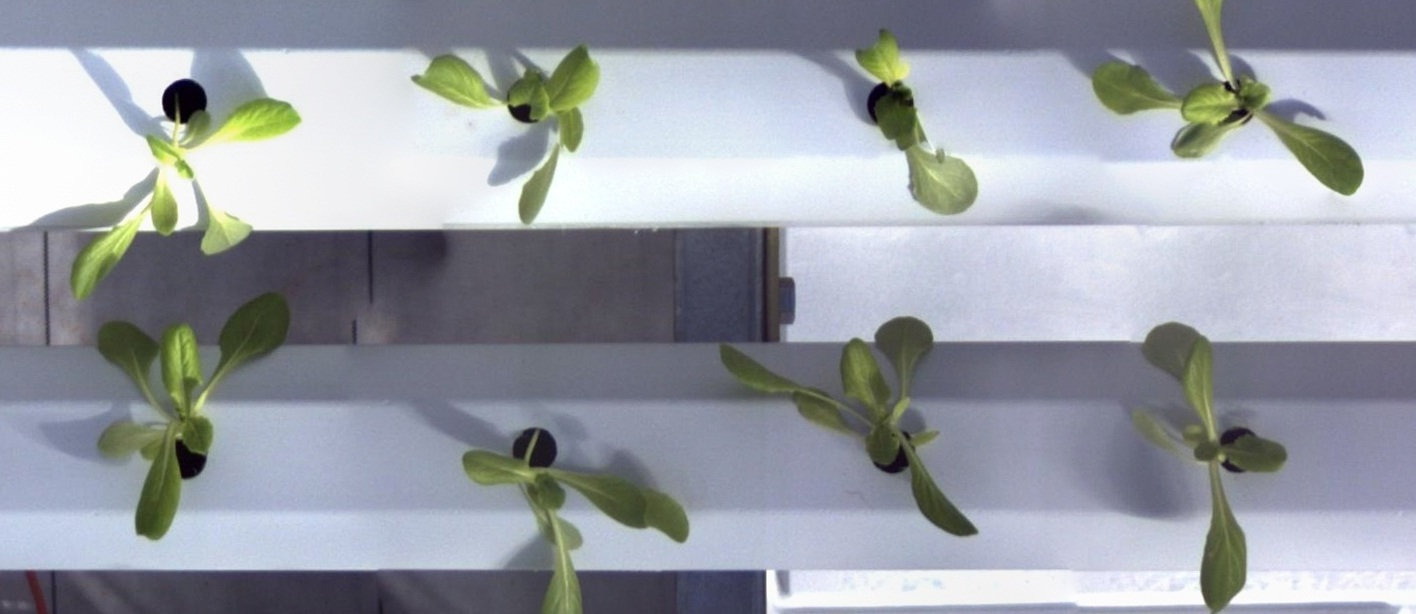
\includegraphics[width=0.5\textwidth]{plt5}}         &
               \subfloat[Color-invariant output.]{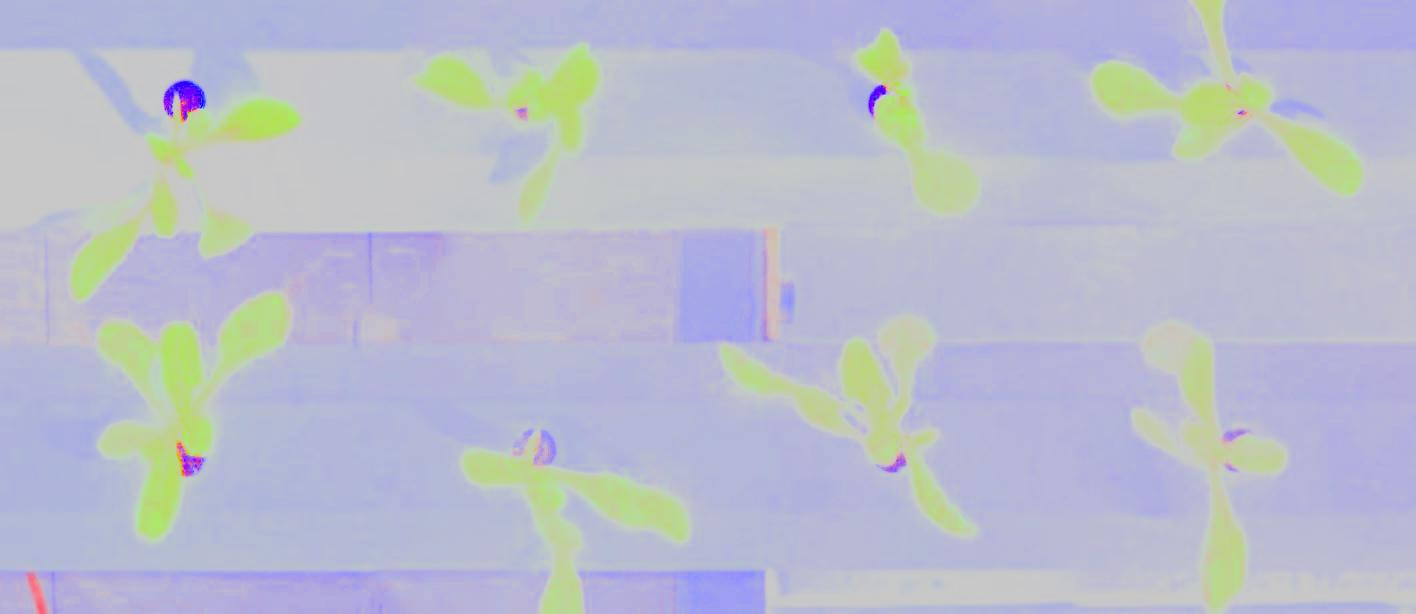
\includegraphics[width=0.5\textwidth]{CIoutput}} \\
               \subfloat[YUV output.]{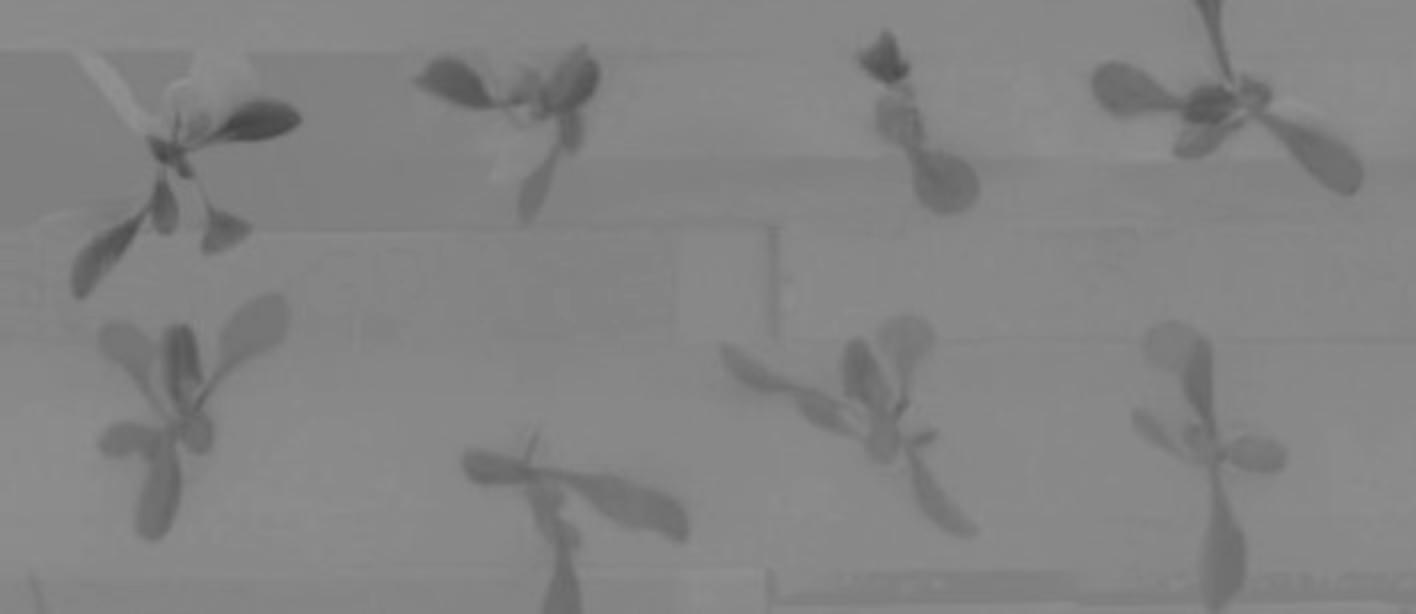
\includegraphics[width=0.5\textwidth]{YUVOutput}}            &
               \subfloat[Grayscale output.]{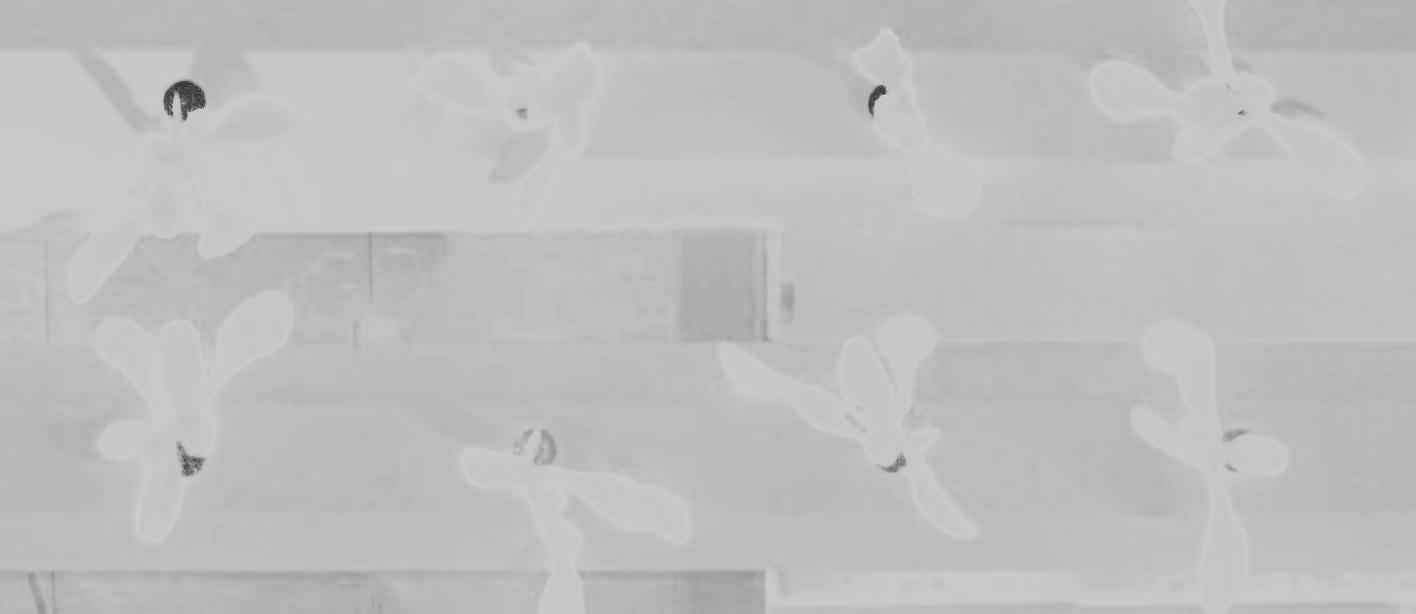
\includegraphics[width=0.5\textwidth]{GrayOutput}}     \\
             \end{tabular}
            \caption{Colorspace transformations of input RGB image.}\label{fig:colorspace}
         \end{figure*}
         %---
         \begin{equation}\label{eq:U}
            U = 0.5 + ( -0.14713 * \textcolor{red}{R} - 0.28886 * \textcolor{green}{G} + 0.43600 * \textcolor{blue}{B})
         \end{equation}
         %---
         \begin{subequations}\label{eq:CI}
            \begin{align}
               CI_{\textcolor{red}{R}}   & = \arctan\left(\frac{\textcolor{red}{R}}{\max(\textcolor{green}{G},\textcolor{blue}{B})}\right)\label{eq:CI_R} \\[2ex]
               CI_{\textcolor{green}{G}} & = \arctan\left(\frac{\textcolor{green}{G}}{\max(\textcolor{red}{R},\textcolor{blue}{B})}\right)\label{eq:CI_G} \\[2ex]
               CI_{\textcolor{blue}{B}}  & = \arctan\left(\frac{\textcolor{blue}{B}}{\max(\textcolor{red}{R},\textcolor{green}{G})}\right)\label{eq:CI_B}
            \end{align}
         \end{subequations}\\
         %---
         \begin{equation}\label{eq:GO}
           G_{out} = 0.299 * CI_{\textcolor{red}{R}} + 0.587 * CI_{\textcolor{green}{G}} + 0.114 * CI_{\textcolor{blue}{B}}
         \end{equation}
         %---
         The original input RGB image with its color-invariant representation, \( U \)-component, and Grayscale outputs are shown in \figurename~\ref{fig:colorspace}.
      %---
      \subsection{Histogram}
         The next process in the algorithm is to calculate the histogram for the Grayscale image. In this process, there are 256 bins to represent each pixel intensity in the histogram. Each pixel intensity bin is the number of pixels in an image that have that same pixel intensity. The histogram is then used in Otsu’s method \cite{Otsu1979} to calculate the threshold. In our CUDA implementation, shared memory was utilized so that the kernel could employ privatization. Each thread block contained a private histogram with 256 bins and would iterate throughout the image using a stride amount calculated using:
         %---
         \begin{equation}\label{eq:stride}
            \mathtt{stride} = \mathtt{blockDim.x} \times \mathtt{gridDim.x}
         \end{equation}
         %---
         The kernel would then atomically increment each private histogram bin based on the pixel intensity read. When the thread has iterated through all valid pixels it will wait for all other threads to finish their iterations. Afterwards the first thread in the thread block will transfer the private histogram values from shared memory to global memory.
      %---
      \subsection{Thresholding and Otsu's Method}
         Otsu's method would then be implemented in order to determine an optimal threshold values for the histogram outputs. Initially, the implemented algorithm calculated the total number of pixels and the weighted sum of pixel intensities using the histograms. The total pixel count and the weighted sum were obtained by iterating through the 256 histogram bins.

         Our algorithm then evaluated the between-class variance for each threshold value. For each threshold, it would separate the histogram into background and foreground, calculating their weights and cumulative sums. The mean intensity for both background and foreground would then be calculated by dividing the cumulative sums by their weights. The variance for each threshold was then computed using the equation for between-class variance \eqref{eqOtsu}.
         %---
         \begin{equation}\label{eqOtsu}
         	\sigma^2_b(t) = w_b(t) \cdot w_f(t) \cdot (\mu_b(t) - \mu_f(t))^2
         \end{equation}
         %---
         The between-class variance in \eqref{eqOtsu} involved the product of the background weights, foreground weights and the square of the difference between the background and foreground means. Our algorithm would then search for the threshold that maximizes the between-class variance. The threshold that was determined to be the optimal value would now be returned to main and would be used when implementing the binarization kernel. The optimal threshold would be determined for both the Grayscale histogram and the YUV histogram.

         In our binarization kernel, the algorithm is implemented so that each CUDA thread was set for processing a single pixel of the image. The global thread index is computed using the block index and thread index, which would correspond to the pixel location in the image.

         Our implemented binarization kernel involved in comparing the pixel intensity against the threshold. If the intensity of a pixel was less than or equal to the threshold, it was labeled as background. If the intensity of a pixel was greater than the threshold, it was labeled as foreground. This labeling in our binarization kernel assisted in distinguishing between shadowed regions and lit areas of the input images. The binarized images would then be returned into global memory for further processing. Both the Greyscale and the YUV image would be binarized using our implemented kernel. After the binarization kernel execution. The binarized images would be produced for both the Greyscale and the YUV Image.
         The output images resulting from the binarization kernel execution are shown below in \figurename~\ref{fig:Binarization}
         %---
         \begin{figure}[h]
         	\centering
         	\subfloat[Grayscale Binarized Output]{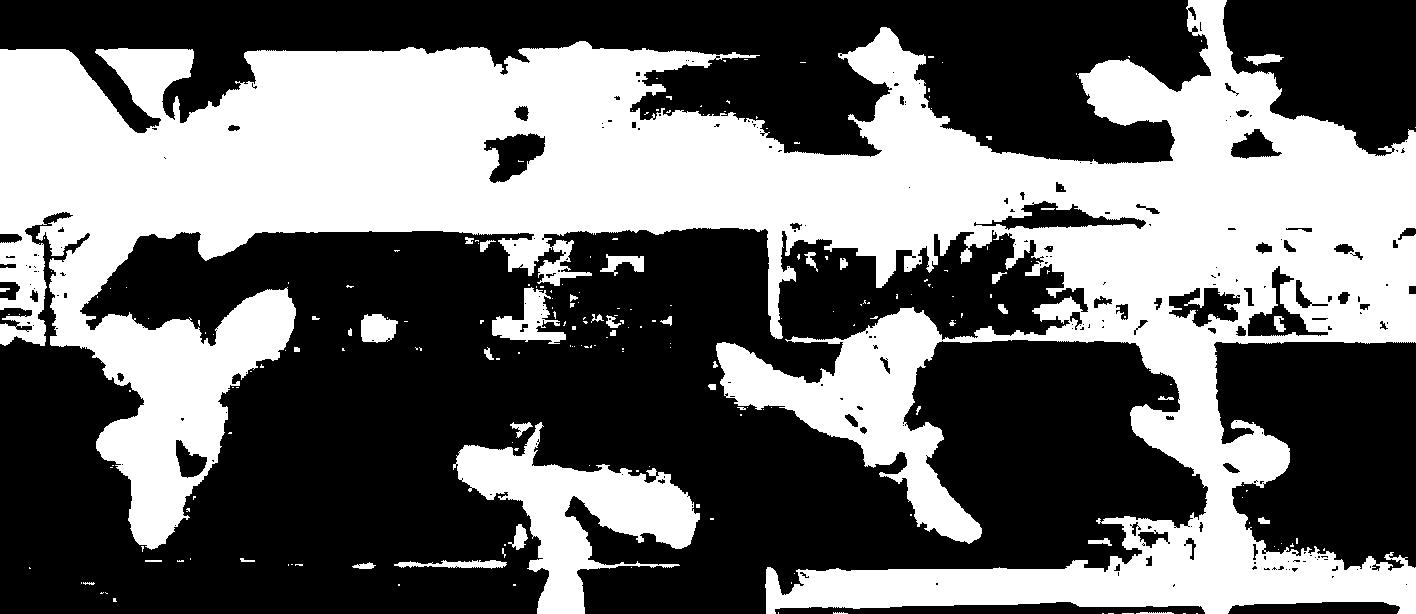
\includegraphics[width=0.5\textwidth]{BinaryOutput_Grey}}

         	\subfloat[YUV Binarized Output]{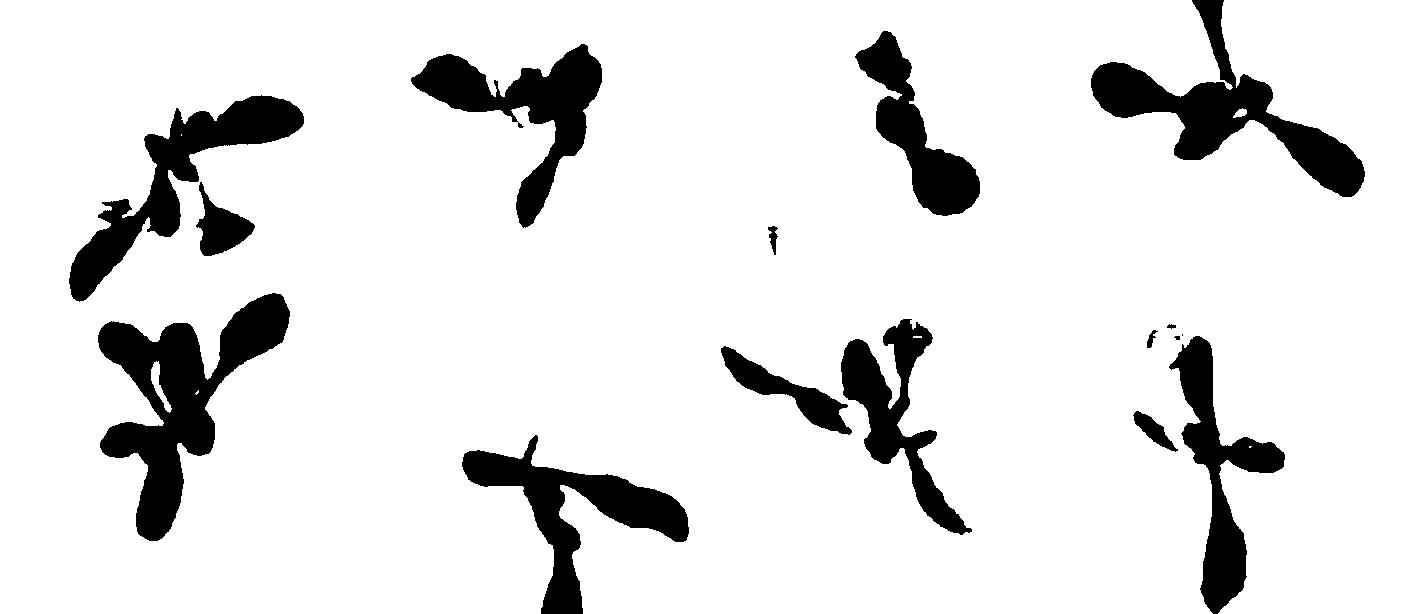
\includegraphics[width=0.5\textwidth]{BinaryOutput_YUV}}
         	\caption{Binarized Output Images.}
         	\label{fig:Binarization}
         \end{figure}

         %---
      %---
      \subsection{Convolution}
         For the convolution procedure, a 5x5 structural element was passed over the input data to filter the input pixels. Each input pixel is first summed with its neighboring pixels, and then multiplied and accumulated according to:
         \begin{equation}\label{eq:Conv}
            f[x,y] * g[x,y] = \sum_{i=1}^{n}\sum_{k=1}^{m}f[i,k] \cdot g[x-i,y-k]
         \end{equation}
         %---
         where the structural element is represented by \( f[x,y]\) and the input image is represented by \( g[x,y] \). In order to optimize the kernel performance, the structural element was declared in constant memory which allowed the NVIDIA compiler to place it into faster cache memory. Careful use of the \texttt{restrict} keyword also allowed the compiler to optimize memory accesses without having to worry about input pointer addresses being aliased with each other. Loop unrolling was also implemented to alleviate the overhead of maintaining and incrementing the various iterator variables.
      %---
      \subsection{Erosion}
         The erosion procedure was quite similar to the convolution procedure, but in a more restricted environment. The simplicity of the erosion morphological operation allowed for a more aggressive optimization approach than what was available for the convolution kernel. Instead of simply unrolling the loops mentioned previously in the convolution kernel, the erosion kernel was able to eliminate the loops entirely. Furthermore, the final pixel value being calculated was determined to have the same truth table as a digital logic AND gate, so the potential for control divergence was completely eliminated by replacing the if condition with a simple bitwise AND operation.
      %---
      \subsection{Result Integration}
         The last process of the algorithm is integration, where the eroded shadow and light mask are used to calculate the RGB ratios. To calculate these ratios, the pixel intensities for the original input image and eroded mask are multiplied and then accumulated, which provides the numerator for the ratio. Then the sum of the pixel intensities for eroded mask images is also calculated, which provides the denominator for the ratio.
         %---
         \begin{subequations}\label{eqInte}
         	\begin{align}
         		\textcolor{red}{R}   & = \left(\frac{RR + 1}{((1 - S) \times RR + 1) \times IR}\right)\label{eqInte_R} \\[2ex]
         		\textcolor{green}{G} & = \left(\frac{RG + 1}{((1 - S) \times RG + 1) \times IG}\right)\label{eqInte_G} \\[2ex]
         		\textcolor{blue}{B}  & = \left(\frac{RB + 1}{((1 - S) \times RB + 1) \times IB}\right)\label{eqInte_B}
         	\end{align}
         \end{subequations}
         %---
         Afterwards the RGB ratios, smooth mask image from convolution, and input image are used to generate the final output image with shadows removed using \eqref{eqInte_R}, \eqref{eqInte_G}, and \eqref{eqInte_B}. In the equations RR is the red ratio, RG is the green ratio, and RB is the blue ratio. The IR, IG, and IB variables are the original input RGB pixel values. The S variable is the pixel value for the smooth mask image from the convolution process.
         In our CUDA implementation, there are three kernels used in the integration process. The first kernel is used to calculate the numerator value for the RGB ratios. In the kernel, a private sum value is declared in shared memory to calculate the sum of the input image multiplied by the eroded grayscale mask. Each thread uses the stride amount shown in \eqref{eq:stride}, to iterate through the image and atomically accumulate the sum in the private sum values in shared memory for the red, green, and blue channels. The first thread in a block then transfers the private RGB sum values to global memory.
         The second kernel is like the first kernel, where a private sum is declared in shared memory. The kernel calculates the sum of pixel intensities for the eroded grayscale shadow and light mask which is used as the denominator for the RGB ratio values.
         The results from the first and second kernel are then divided in the host code to generate the RGB ratio values which are used by the third kernel to generate the final output image with shadows removed.
         In the third kernel, only global memory is used to calculate the result image, which uses the equations in \eqref{eqInte_R}, \eqref{eqInte_G}, and \eqref{eqInte_B} to generate the RGB values for the final output image.
   %---
   \section{Evaluation and Validation}
      %---
      \begin{figure*}[!t]
         \centering
         \begin{tabular}{cc}
         \subfloat[Original RGB image.]{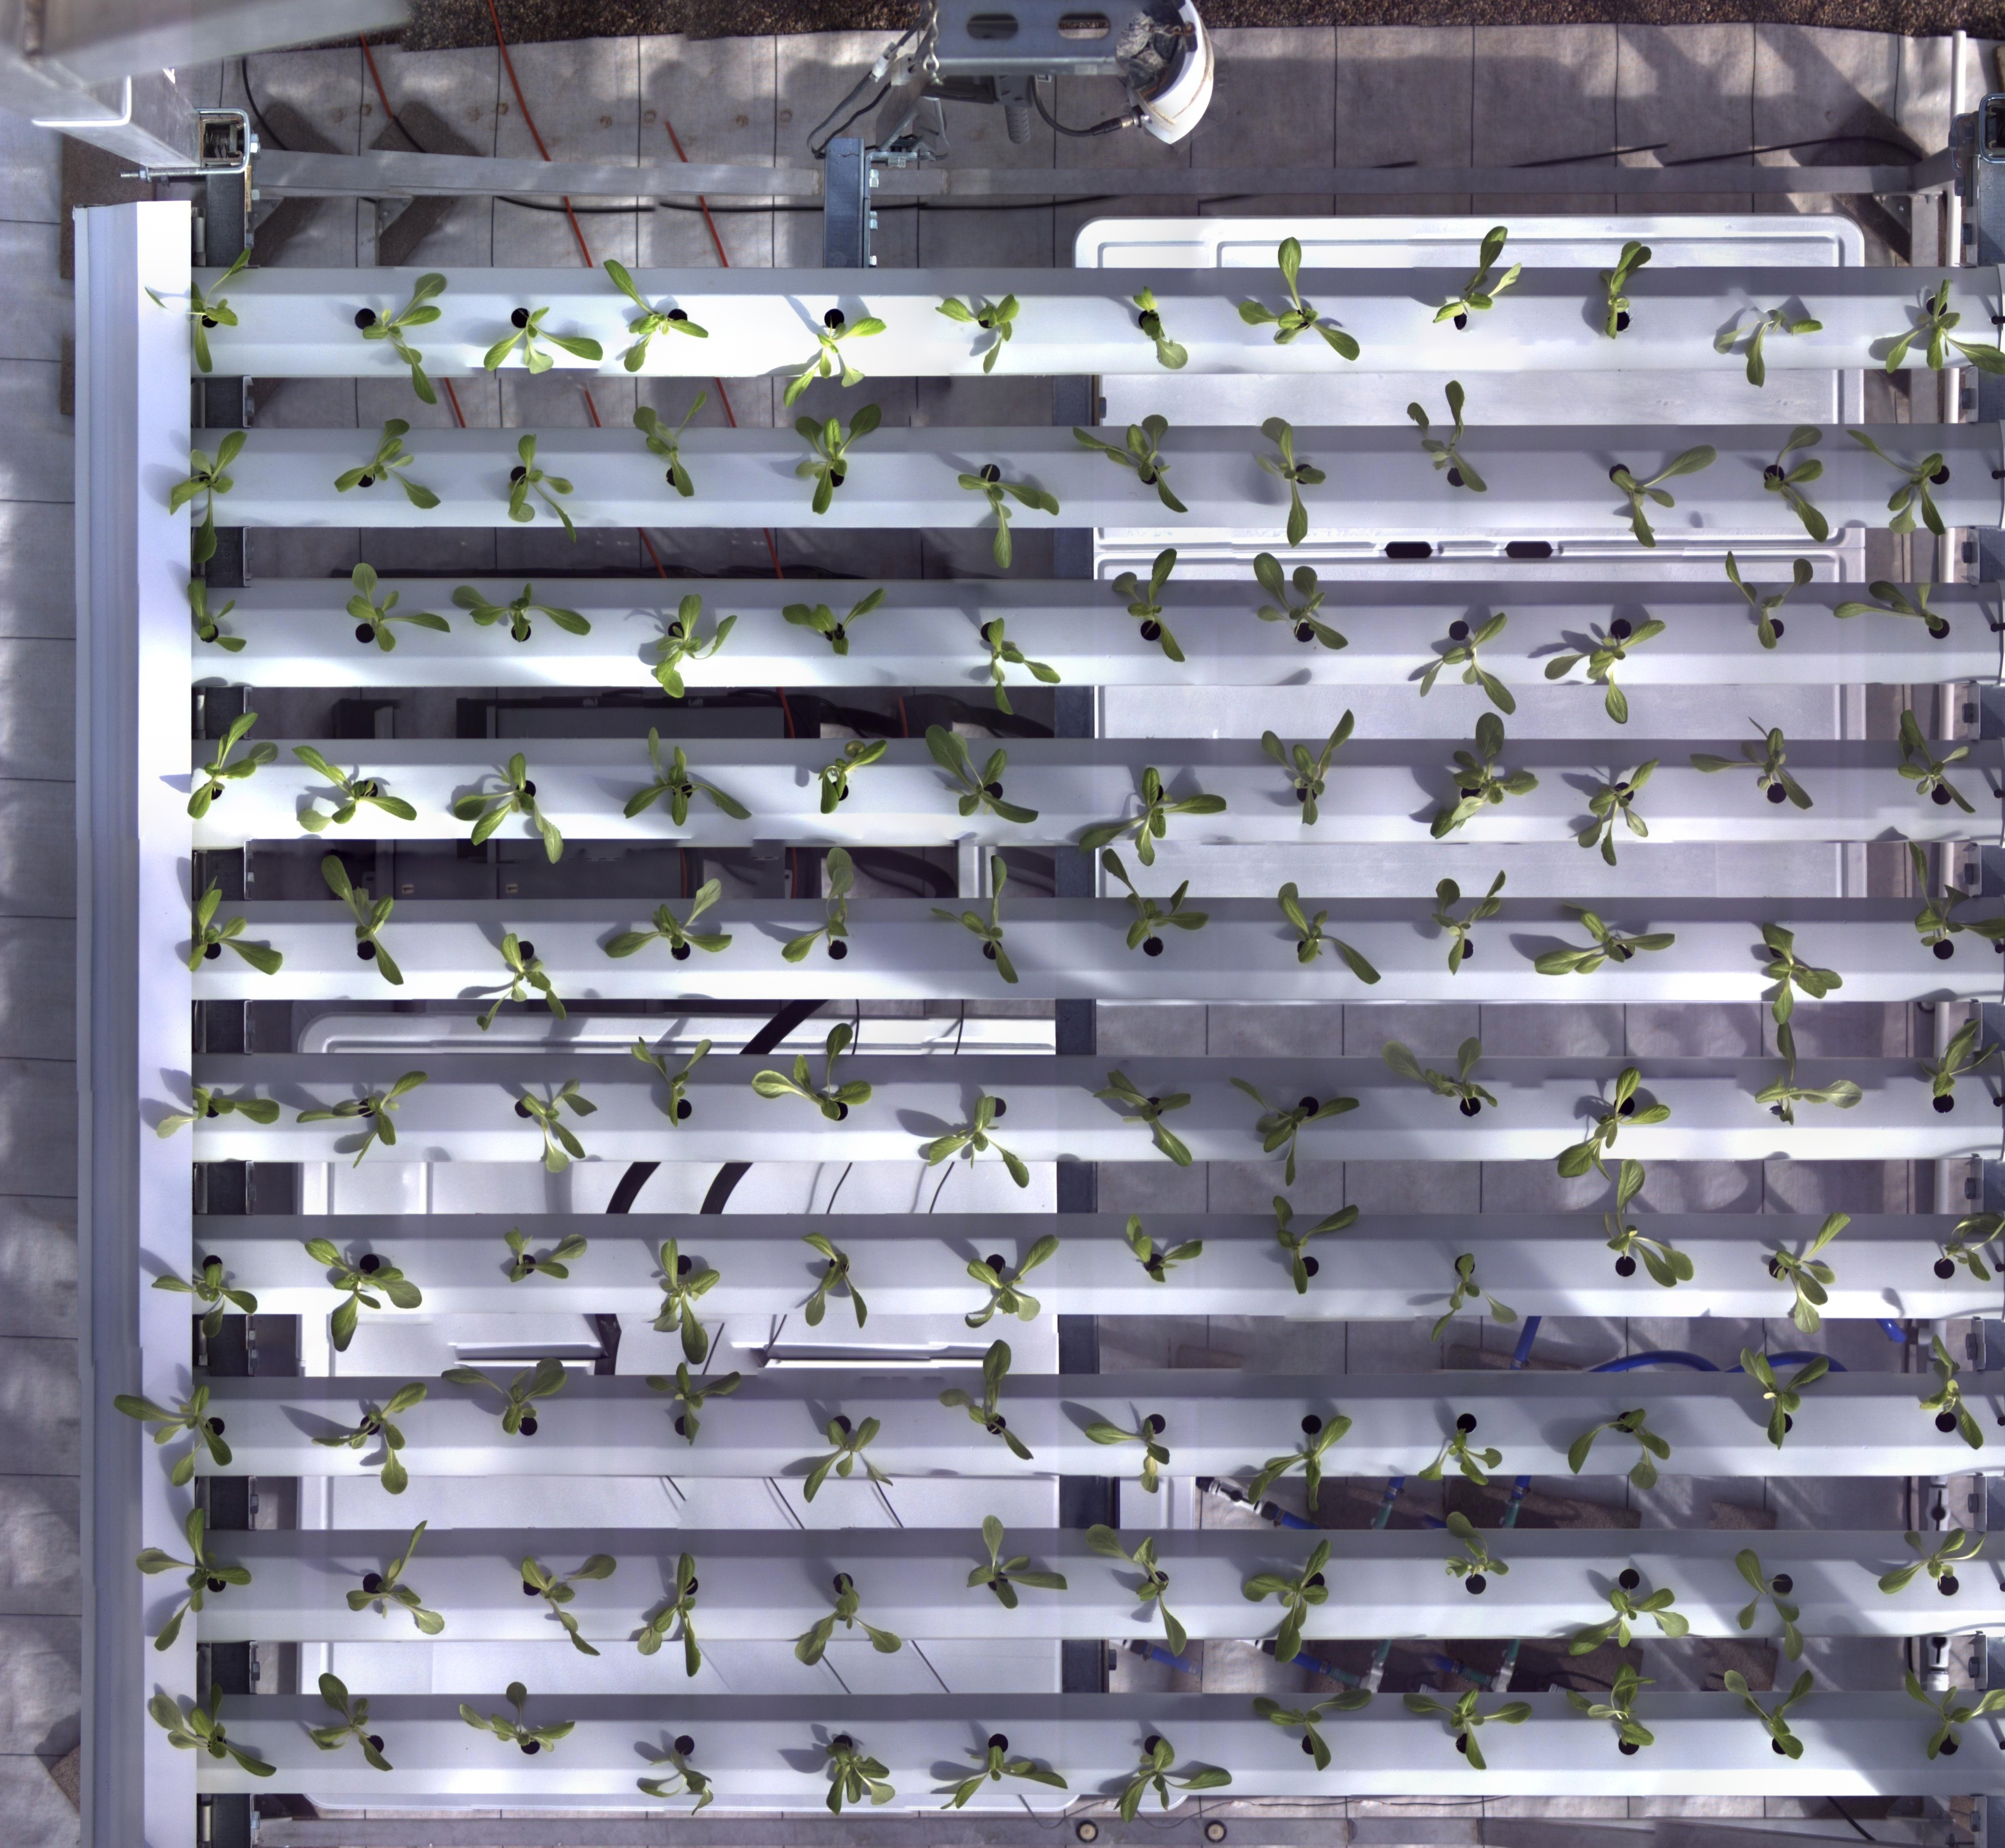
\includegraphics[width=0.5\textwidth]{plt}}         &
         \subfloat[Result Output Image.]{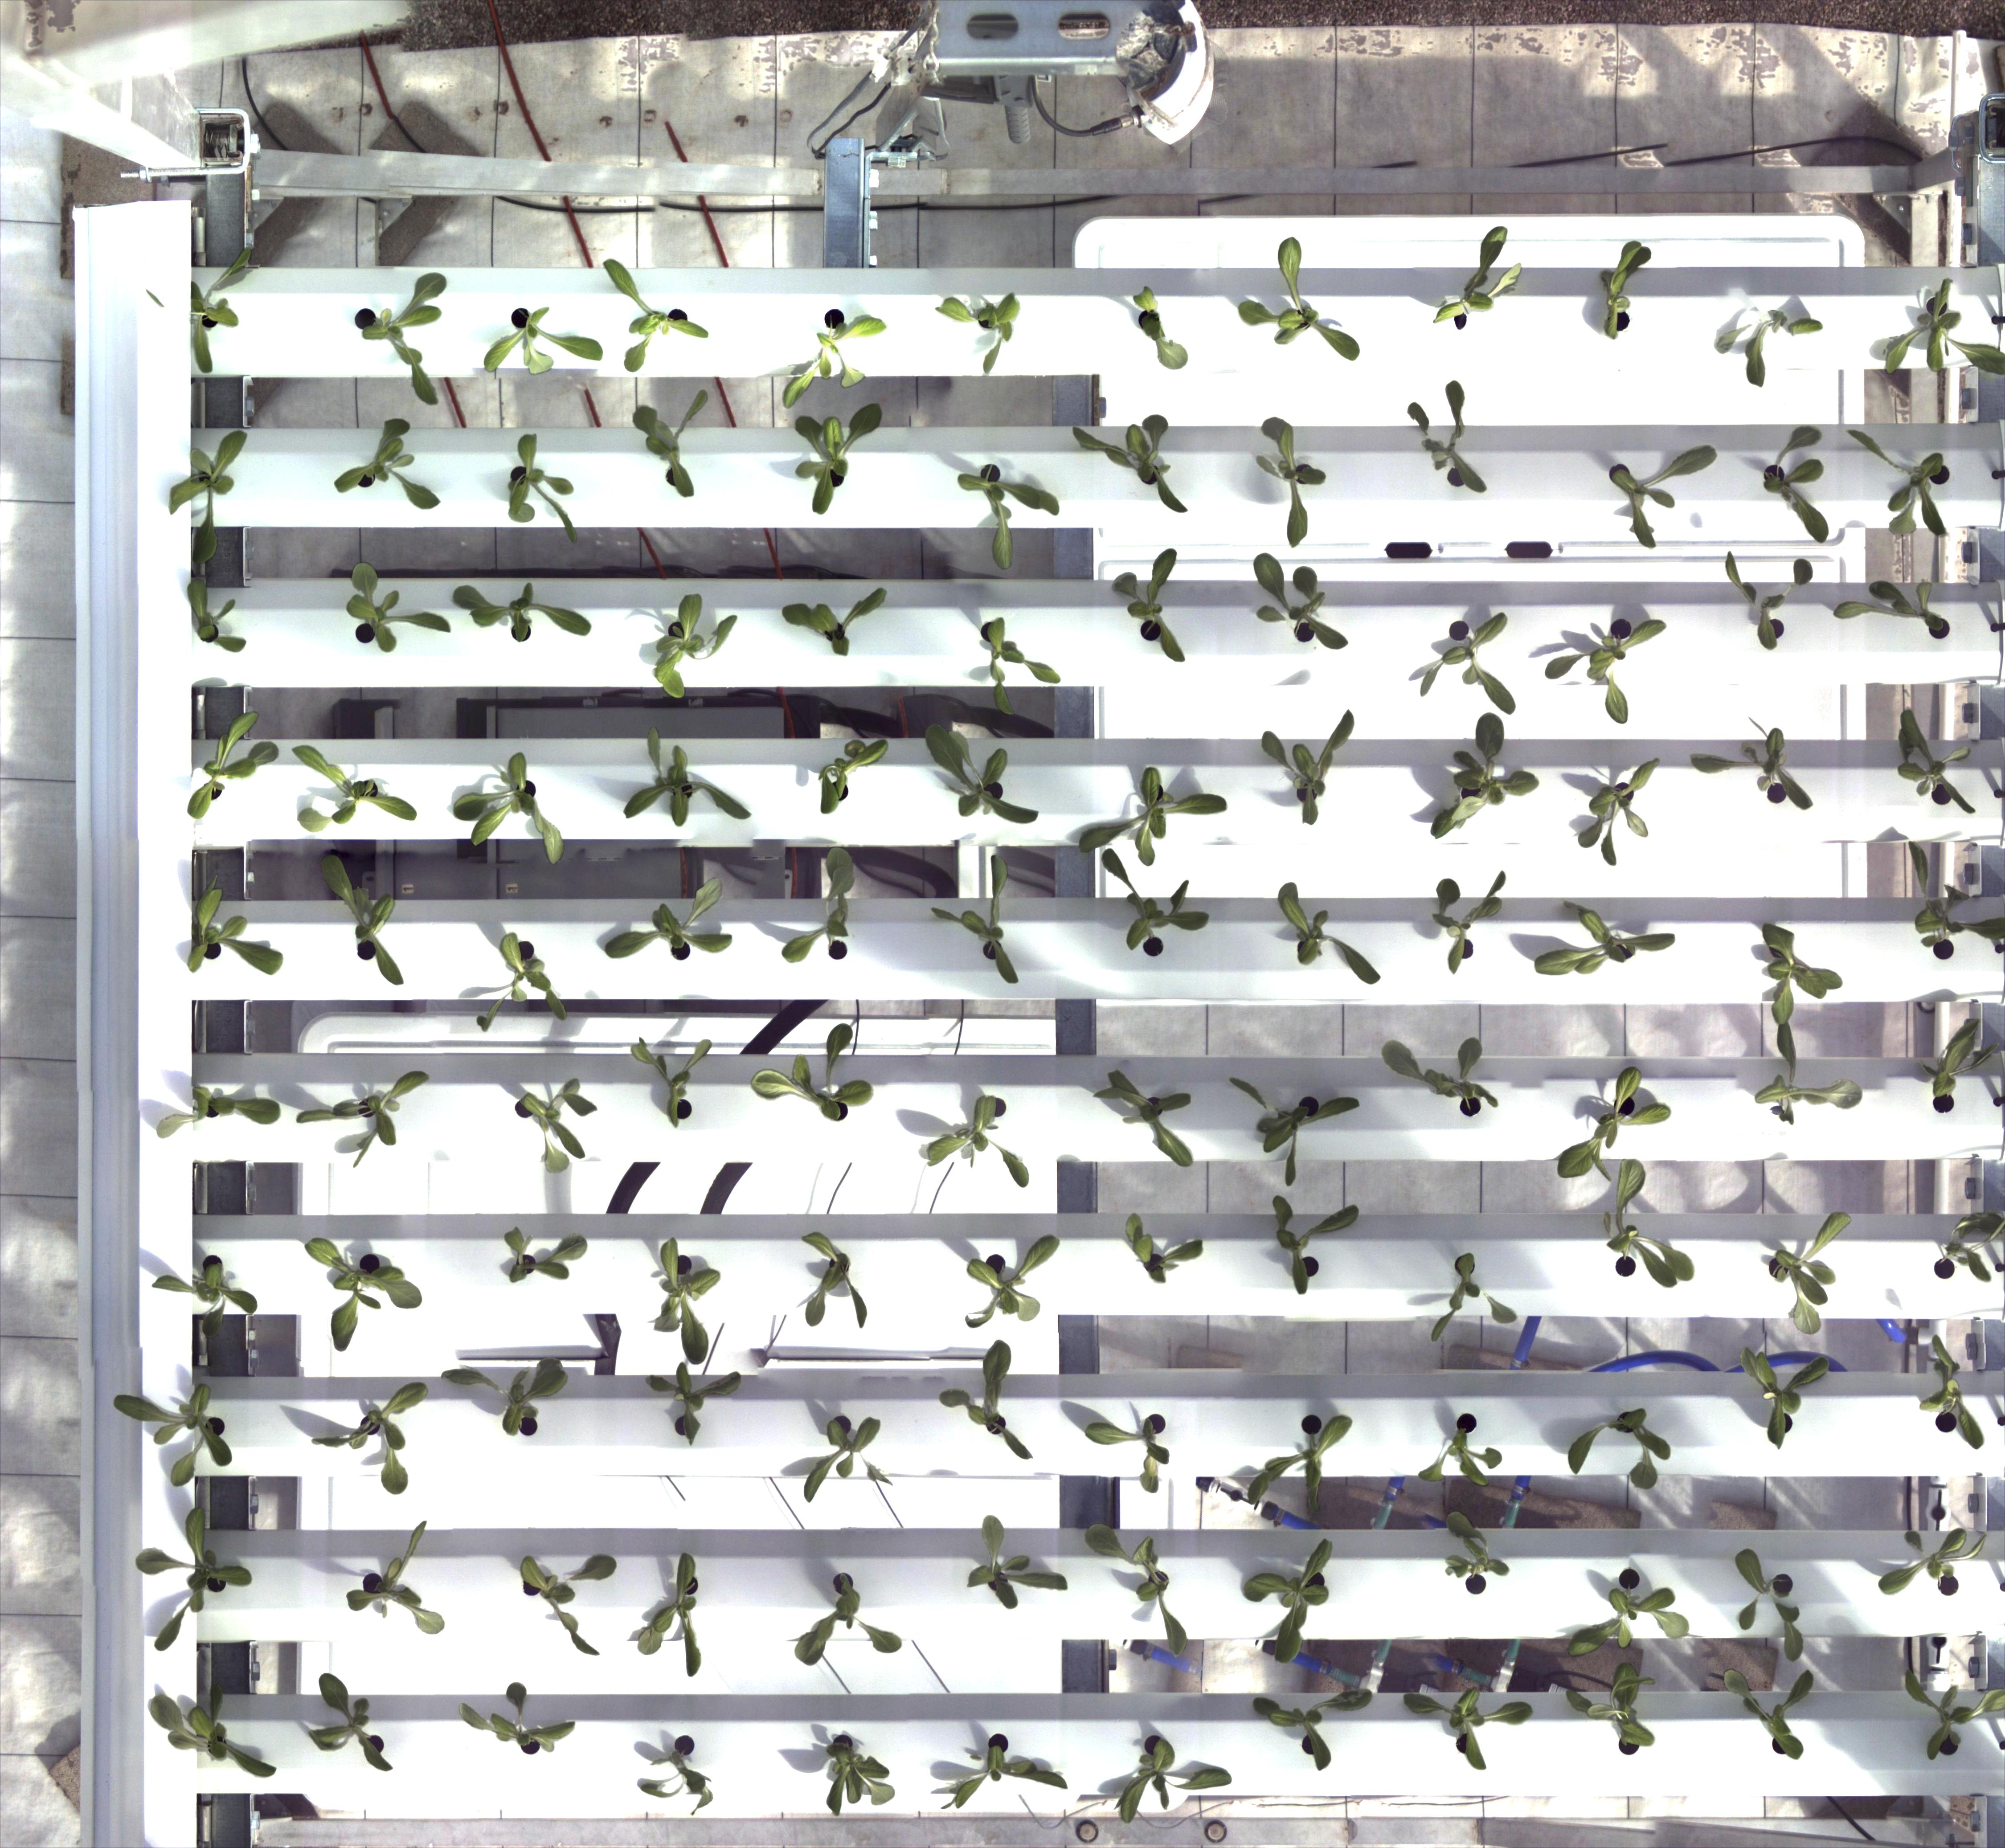
\includegraphics[width=0.5\textwidth]{Result5}} \\
         \end{tabular}
         \caption{Comparison of Original and Output Image.}\label{fig:result}
      \end{figure*}
      %---
      \begin{table}[!t]
      	\renewcommand{\arraystretch}{1.3}
      	\caption{Execution Time Data for 1548x976 Image}
      	\label{table_example}
      	\centering
      	\begin{tabular}{c|c|c|c}
      		\hline
      		\bfseries Kernel & Serial Time(us) & CUDA Time(us) & Speedup \\
      		\hline\hline
      		Colorspace  & 107160.00 & 862.46 & 124.25 \\
      		\hline
      		Histogram(Grayscale) & 430.04 & 552.90 & 0.78 \\
      		\hline
      		Histogram(YUV) & 277.05 & 552.97 & 0.50 \\
      		\hline
      		Binarize(Shadow-Gray) & 2360.20 & 79.14 & 14.90 \\
      		\hline
      		Binarize(Light-Gray) & 2360.20 & 79.26 & 14.90 \\
      		\hline
      		Binarize(Light-YUV) & 1863.80 & 79.12 & 23.56 \\
      		\hline
      		Convolution & 2138.40 & 296.51 & 7.21 \\
      		\hline
      		Erosion(Light) & 3222.00 & 79.34 & 40.61 \\
      		\hline
      		Erosion(Shadow) & 3269.80 & 79.37 & 41.20 \\
      		\hline
      		Mapping(Shadow) & 10862.00 & 3021.57 & 3.59 \\
      		\hline
      		Mapping(Light) & 10380.00 & 3539.34 & 2.93 \\
      		\hline
      		Mask Comb.(Shadow) & 182.75 & 1740.77 & 0.10 \\
      		\hline
      		Mask Comb.(Light) & 175.68 & 2254.34 & 0.08 \\
      		\hline
      		Result Image & 28233.00 & 343.42 & 82.21 \\
      		\hline
      		Total: & 170554.71 & 13560.54 & 12.58 \\
      	\end{tabular}
      \end{table}

      \begin{table}[!t]
      	\renewcommand{\arraystretch}{1.3}
      	\caption{Execution Time Data for 4500x4148 Image with Floating Point Optimizations}
      	\label{table_example}
      	\centering
      	\begin{tabular}{c|c|c|c}
      		\hline
      		\bfseries Kernel & Serial Time(us) & CUDA Time(us) & Speedup \\
      		\hline\hline
      		Colorspace  & 1659000.00 & 3916.96 & 423.54 \\
      		\hline
      		Histogram(Grayscale) & 5662.90 & 6771.49 & 0.84 \\
      		\hline
      		Histogram(YUV) & 1281.44 & 6771.26 & 0.19 \\
      		\hline
      		Binarize(Shadow-Gray) & 26413.00 & 960.26 & 13.76 \\
      		\hline
      		Binarize(Light-Gray) & 26413.00 & 959.42 & 13.76 \\
      		\hline
      		Binarize(Light-YUV) & 24323.00 & 959.84 & 25.34 \\
      		\hline
      		Convolution & 46756.00 & 3625.15 & 12.90 \\
      		\hline
      		Erosion(Light) & 47495.00 & 968.13 & 49.06 \\
      		\hline
      		Erosion(Shadow) & 33219.00 & 969.31 & 34.27 \\
      		\hline
      		Mapping(Shadow) & 140080.00 & 35933.22 & 3.90 \\
      		\hline
      		Mapping(Light) & 147100.00 & 43965.70 & 3.35 \\
      		\hline
      		Mask Comb.(Shadow) & 7256.30 & 20393.18 & 0.36 \\
      		\hline
      		Mask Comb.(Light) & 7151.00 & 27955.90 & 0.26 \\
      		\hline
      		Result Image & 345030.00 & 4195.04 & 82.25 \\
      		\hline
      		Total: & 2490767.64 & 158344.86 & 15.73 \\
      		\hline
      	\end{tabular}
      \end{table}
      %---
      The results in this section were obtained using a computer that had an Intel Core i7 12800H CPU with an operating frequency of 2.4 GHz. The GPU used to obtain the CUDA executions times was the NVIDIA RTX A2000 Laptop GPU with 20 streaming multiprocessors and a total of 3,328 Ampere-based CUDA cores.
      %---
      \subsection{Colorspace Transformation}
         In our colorspace kernel, we were able to achieve a speedup factor of 124x. Each thread in the kernel performed the transformation on one pixel in the original image. Also like in \cite{Akoglu}, only the U component in the YUV transformation was calculated since the Y and V components were not needed. Also like \cite{Akoglu}, we used the atanf() function from the CUDA library which reduced the calculation time. Since each thread works on subsequent pixel, the memory accesses also work on consecutive locations so there is a form of memory coalescing which increases the performance of the kernel. Some improvements that could have been made to our CUDA source code were to put a type specifier on the floating point literals, which we observed having around 3x to 4x speedup compared to our implementation based on results from the NVIDIA profiler tool. The results from the NVIDIA profiler tool also showed the memory throughput being 31.62\%. The reason for this low throughput was the large amount of global memory accesses which take a longer time in comparison to shared memory or constant memory accesses. In the kernel, there were 3 global memory reads for the input image and 5 global memory writes for the color invariant, U component, and grayscale image.
      %---
      \subsection{Histogram}
         Our histogram kernel performed worse than the MATLAB serial implementation. This was also the case in Richter et al. \cite{Akoglu} as well. Our kernel performed an average of 0.65x of the MATLAB serial implementation. In our kernel, each loop has 1 global memory read, 1 atomic addition to shared memory, and 1 integer addition. The number of loops is dependent on the image size. Each thread also transfers the private histogram bin values to global memory. According to the NVIDIA profile tool, the histogram kernel has a compute throughput of 45.63\% and a memory throughput of 31.64\%. The reason for the low throughput may be due to the large number of writes to shared and global memory. Also, the memory accesses are not coalesced, which also affects the performance of the kernel.
      %---
      \subsection{Thresholding and Otsu’s Method}
         Our Otsu’s thresholding method was implemented using a CPU bound function while the binarization kernel was implemented using CUDA architecture. In our binarization kernel, we were able to achieve a speedup factor of 14.90x for the Grayscale binarization and a 23.90x factor for the YUV Image binarization for the 1548x976 dimensions. For the 4500x4148 images, we were able to achieve a speedup factor of 13.75x for the Grayscale binarization and a 25.34x factor for the YUV Image binarization.  Each thread in our kernel performed binarization on each pixel in the inputting images. Compared to our MATLAB execution, for 1548x976 dimensions the execution time for Grayscale binarization was 2360\micro s on MATLAB and 79\micro s on CUDA. For YUV, our MATLAB execution time was 1863\micro s and 79.33\micro s on CUDA. As observed, MATLAB execution was significantly slower than the CUDA implementation.  For 4500x4148 dimensions the execution time for Grayscale binarization was 26413\micro s on MATLAB and 959\micro s on CUDA. For YUV, our MATLAB execution time was 24323\micro s and 959\micro s on CUDA. As observed, MATLAB execution was significantly slower than the CUDA implementation. Our CUDA implemented kernel had a significantly fast execution time primarily due to the parallelism that was offered by our GPU, while our MATLAB code processed the binarizations in a sequential manner on the CPU. For our CUDA kernel, the architecture performs the binarization operation concurrently across many pixels where each of the threads can binarize a pixel simultaneously, which significantly reduces the time to process the images. Comparing the different dimensions, CUDA processing is more advantageous for larger scale images since the high throughput of image data would need to be processed.
      %---
      \subsection{Convolution and Erosion}
         The convolution and erosion kernels had substantial performance gains over the serial MATLAB implementation across the entire range of input images tested. For the convolution kernel, the realized speedup varied from 7x—10.5x for the smaller images, and just under 13x for the large 4500x4148 pixel image. The erosion kernels performed much better than the convolution kernel, having a minimum average speedup of approximately 25x for the smaller images, to nearly 50x speedup for the large 4500x4148 pixel image.
      %---
      \subsection{Integration}
         The three kernels that make up the integration process are the image mapping, image mask combination, and the result image kernel. The total speed up for the integration process was approximately 4.5x, with the result image kernel performing the best out of the three. Despite the result image kernel performing the best compared to MATLAB, there were still improvements that could be made. The NVIDIA profiler tool showed that a 59\% speedup could occur if there were no uncoalesced memory accesses. The profiling tool also revealed a 24.23\% compute throughput for the result image kernel as well, which is due to the various multiplications, additions, and division operations having to be used. In the kernel there were 6 floating point additions, 6 floating point multiplications, 3 floating point subtractions, and 1 floating point division which contributes to the low compute throughput. There were also 9 global memory reads and 3 global memory writes that contributed to the performance.
         Our image mapping kernel also showed a speed up factor of around 3x in comparison to MATLAB. The kernel had 6 global reads and 3 atomic additions to shared memory for each loop iteration. There were also 3 floating point multiplications that contributed to the execution time of the kernel. The first thread of the thread block would also transfer the data from shared memory to global memory using the atomic addition operation. The NVIDIA profiler tool also showed a 73\% compute and memory throughput for the image mapping kernel. Since the kernel is always reading the same image mask value from memory, the number of global reads could of have been reduced to 4, which would help with the memory throughput.
         The image mask combination kernel performed the worst compared to MATLAB, where the CUDA kernel ran slower at around a factor of 0.1x. The MATLAB implementation seemed to perform well in which it only took around 180\micro s to compute the sum of the image mask pixel array compared to our CUDA kernel which took an average of 2000\micro s. The compute and memory throughput were around 70\%. There is only 1 global read and 1 atomic addition to shared memory for each loop. Also, only the first thread in a block uses an atomic addition to transfer the private sum value to global memory. The speed up factor did increase slightly with a larger image size, since the MATLAB serial implementation has to execute more operations and the CUDA program only launches more threads which are running in parallel, which does not increase the execution time.
      %---
      \subsection{Total Speedup}
         As can be seen in Table I, our CUDA program had a total speedup of 12.57x for a 1548x976 image. If we were to add type specifiers to our floating-point literals, we would have a speed up factor of 15.73x which is shown in Table II. Both tables show the execution times and speed up factors relative to the MATLAB serial implementation for each kernel. Some kernels were executed multiple times but with different inputs, which is accounted for in Table I and Table II. \figurename~\ref{fig:result} shows the comparison between the original image and the shadowless image.
   %---
   \section{Conclusion}
		 Our project successfully demonstrated the advantages of using CUDA C++ for the efficient detection and removal of shadows from the inputted images. By using the capabilities of GPUs, our implementation managed to process images much faster than traditional methods such as MATLAB, and in result showed how valuable parallel computing can be for complex image processing tasks.

		 For future work, there are several ways this project could be further improved and expanded. Initially, optimizing the kernels already implemented would be beneficial in terms of efficiency. Another potential area for future development would be optimizing memory usage to make the processes more efficient, which would be advantageous for processing images with a larger amount of pixel data.
   %---
   %   \bibliography{ECE569_ProjectReferences}
   %   \bibliographystyle{IEEETran}
   % Generated by IEEEtran.bst, version: 1.14 (2015/08/26)
   \begin{thebibliography}{10}
      \providecommand{\url}[1]{#1}
      \csname url@samestyle\endcsname
      \providecommand{\newblock}{\relax}
      \providecommand{\bibinfo}[2]{#2}
      \providecommand{\BIBentrySTDinterwordspacing}{\spaceskip=0pt\relax}
      \providecommand{\BIBentryALTinterwordstretchfactor}{4}
      \providecommand{\BIBentryALTinterwordspacing}{\spaceskip=\fontdimen2\font plus
         \BIBentryALTinterwordstretchfactor\fontdimen3\font minus
         \fontdimen4\font\relax}
      \providecommand{\BIBforeignlanguage}[2]{{%
            \expandafter\ifx\csname l@#1\endcsname\relax
            \typeout{** WARNING: IEEEtran.bst: No hyphenation pattern has been}%
            \typeout{** loaded for the language `#1'. Using the pattern for}%
            \typeout{** the default language instead.}%
            \else
            \language=\csname l@#1\endcsname
            \fi
            #2}}
      \providecommand{\BIBdecl}{\relax}
      \BIBdecl

      \bibitem{GpuGems3}
      \BIBentryALTinterwordspacing
      N.~Goodnight. \BIBforeignlanguage{en-US}{{Part VI: GPU Computing}}. GPU Gems 3.
      NVIDIA Corporation. [Online]. Available:
      \url{https://developer.nvidia.com/gpugems/gpugems3/part-vi-gpu-computing}
      \BIBentrySTDinterwordspacing

      \bibitem{Akoglu}
      E.~Richter, R.~Raettig, J.~Mack, S.~Valancius, B.~Unal, and A.~Akoglu,
      ``Accelerated shadow detection and removal method,'' in \emph{2019 IEEE/ACS
         16th International Conference on Computer Systems and Applications (AICCSA)},
      Nov 2019, pp. 1--8.

      \bibitem{Wu2020}
      \BIBentryALTinterwordspacing
      M.~Wu, R.~Chen, and Y.~Tong, ``\BIBforeignlanguage{en}{Shadow {Elimination}
         {Algorithm} {Using} {Color} and {Texture} {Features}},''
      \emph{\BIBforeignlanguage{en}{Computational Intelligence and Neuroscience}},
      vol. 2020, p. e2075781, Jan. 2020. [Online]. Available:
      \url{https://www.hindawi.com/journals/cin/2020/2075781/}
      \BIBentrySTDinterwordspacing

      \bibitem{Qu2023}
      \BIBentryALTinterwordspacing
      H.~Qu, C.~Tong, and W.~Liu, ``\BIBforeignlanguage{en}{Image shadow removal
         algorithm guided by progressive attention mechanism},''
      \emph{\BIBforeignlanguage{en}{Signal, Image and Video Processing}}, vol.~17,
      no.~5, pp. 2565--2571, Jul. 2023. [Online]. Available:
      \url{https://doi.org/10.1007/s11760-022-02473-z}
      \BIBentrySTDinterwordspacing

      \bibitem{Otsu1979}
      N.~Otsu, ``A threshold selection method from gray-level histograms,''
      \emph{IEEE Transactions on Systems, Man, and Cybernetics}, vol.~9, no.~1, pp.
      62--66, Jan 1979.

      \bibitem{Zhang2015}
      L.~Zhang, Q.~Zhang, and C.~Xiao, ``Shadow remover: Image shadow removal based
      on illumination recovering optimization,'' \emph{IEEE Transactions on Image
         Processing}, vol.~24, no.~11, pp. 4623--4636, 2015.

      \bibitem{Dexon}
      \BIBentryALTinterwordspacing
      (2022, Apr.) \BIBforeignlanguage{en-US}{What are {RGB} and {YUV} color spaces?}
      DEXON Systems. [Online]. Available:
      \url{https://dexonsystems.com/blog/rgb-yuv-color-spaces}
      \BIBentrySTDinterwordspacing

      \bibitem{CUDAv12-4}
      \BIBentryALTinterwordspacing
      (2024, Apr.) {CUDA Toolkit Documentation 12.4 Update 1}. NVIDIA Corporation.
      [Online]. Available:
      \url{https://docs.nvidia.com/cuda/#cuda-toolkit-documentation-v12-4}
      \BIBentrySTDinterwordspacing

      \bibitem{Dynamsoft}
      \BIBentryALTinterwordspacing
      (2019, May) \BIBforeignlanguage{en}{Image {Processing} 101 {Chapter} 1.3:
         {Color} {Space} {Conversion}}. Dynamsoft Corporation. [Online]. Available:
      \url{https://www.dynamsoft.com/blog/insights/image-processing/image-processing-101-color-space-conversion/}
      \BIBentrySTDinterwordspacing

      \bibitem{Le2019}
      H.~Le and D.~Samaras, ``Shadow removal via shadow image decomposition,'' in
      \emph{2019 IEEE/CVF International Conference on Computer Vision (ICCV)},
      2019, pp. 8577--8586.

   \end{thebibliography}
   %---
\end{document}
